%%%%%%%%%%%%%% 
% Fichero: EjFigx
% Autor: J. Salido (http://www.uclm.es/profesorado/jsalido)
% Fecha: febrero, 2017
% Descripción: Ejemplo básico de inclusión de figuras.
% Ejemplo del curso: “LaTeX esencial para preparación de TFG, Tesis
% y otros documentos académicos” (Esc. Sup. Informática-UCLM)
%%%%%%%%%%%%%%




%%%%%%%%%%%%%%
% Preámbulo del documento
%%%%%%%%%%%%%%
\documentclass[11pt,a4paper]{article} 
\usepackage[utf8]{inputenx} 
\usepackage[spanish]{babel} 
\usepackage[left=2cm,right=2cm,top=2cm,bottom=2cm]{geometry} % Márgenes 

% Tipografía
\usepackage{newpxtext}
\usepackage{newpxmath}

\usepackage{marvosym}
\usepackage{pifont} % Generación de símbolos especiales
\usepackage{textcomp}

\usepackage[T1]{fontenc} % Codificación de salida    
\usepackage{microtype} % Mejoras de microtipografía en la obtención de PDF (sólo para pdflatex)
\usepackage{url} % Para escritura de URL
\urlstyle{sf}

% Generación de hiperenlaces
\usepackage[pdftex,breaklinks,colorlinks,
			citecolor=blue, % Color de la citas
			urlcolor=blue, % Color de las URL
			bookmarksnumbered=true, % Incluye números en bookmarks
			pdftitle={Fundamentos de LaTeX para principiantes},
			pdfauthor={Jesús Salido},
			pdfsubject={LaTeX}]{hyperref}

% Listas
\usepackage{paralist} % Mayor control de listas
\usepackage{multicol} % Elementos en varias columnas

% Gráficos
\usepackage{tikz}     	% Creación de figuras nativas en LaTeX
\usepackage{graphicx} 	% Inclusión de figuras y escalado de cajas

\usepackage[margin=10pt,labelfont=bf]{caption}
\usepackage[margin=10pt,font=small,labelfont=bf]{subcaption}	% Inclusión de subfiguras
\usepackage{rotating}	% Rotación de figuras
\usepackage{pgf}		% Inclusión de figuras con comandos LaTeX 

% Declaración del path donde están los archivos de figuras. 
% También se puede incluir el path en el nombre del fichero.
\graphicspath{{../figs/}}  
\DeclareGraphicsExtensions{.pdf,.png,.jpg}
% Lista de extensiones de ficheros por orden de precedencia. De este modo no hace falta indicar la extensión del fichero y en caso de existir dos fichero con el mismos nombre y extensión diferente se emplea el que tiene una extensión con mayor prioridad.




% Con estas instrucciones se ajustan los valores del índice
\setcounter{secnumdepth}{1} % Ajusta el valor del último nivel numerado
\setcounter{tocdepth}{2} %Ajusta el valor del último nivel que aparece en TOC


\author{Jesús Salido}
\title{Inclusión avanzada de figuras en \LaTeX{}}
\date{\today}

%%%%%%%%%%%%%%
% Comienzo del documento
%%%%%%%%%%%%%%
\begin{document}

\maketitle

\begin{abstract}
	Aquí se muestran algunos recursos avanzados para la inclusión de figuras con \LaTeX{}.
\end{abstract}

\tableofcontents
\listoffigures


\section{Subfiguras}
La inclusión de figuras requiere al menos el empleo del paquete \texttt{graphicx} con el que ya se pueden obtener resultados muy aceptables, aunque existen otros paquetes más especializados que facilitan hacer cosas más exóticas, como el paquete \texttt{subcaption}\footnote{Existen otros paquetes para incluir subfiguras como \texttt{subfig} y \texttt{subfigure}, aunque este último ha quedado obsoleto.} para presentar figuras compuestas de varias subfiguras (ver Figs.~\ref{fig:clock} y \ref{fig:lion}). A pesar de la posibilidad del uso del paquete \texttt{subcaption} no se debe descartar la alternativa de la composición externa a \LaTeX{} de las subfiguras y su inclusión en el documento como una figura sencilla (ver Fig.~\ref{fig:2clock}). Esta alternativa hace innecesario el empleo de paquetes dedicados.


% NOTA: Inclusión de subfiguras con paquete "subfigure" ya obsoleto.
%\begin{figure}[hbt]
%	\centering
%	\subfigure[Imagen jpg en color]{
%		\includegraphics[width=5.5cm]{clockCR}
%		\label{fig:clockCR}
%	}
%	\subfigure[Imagen jpg en niveles de gris]{
%		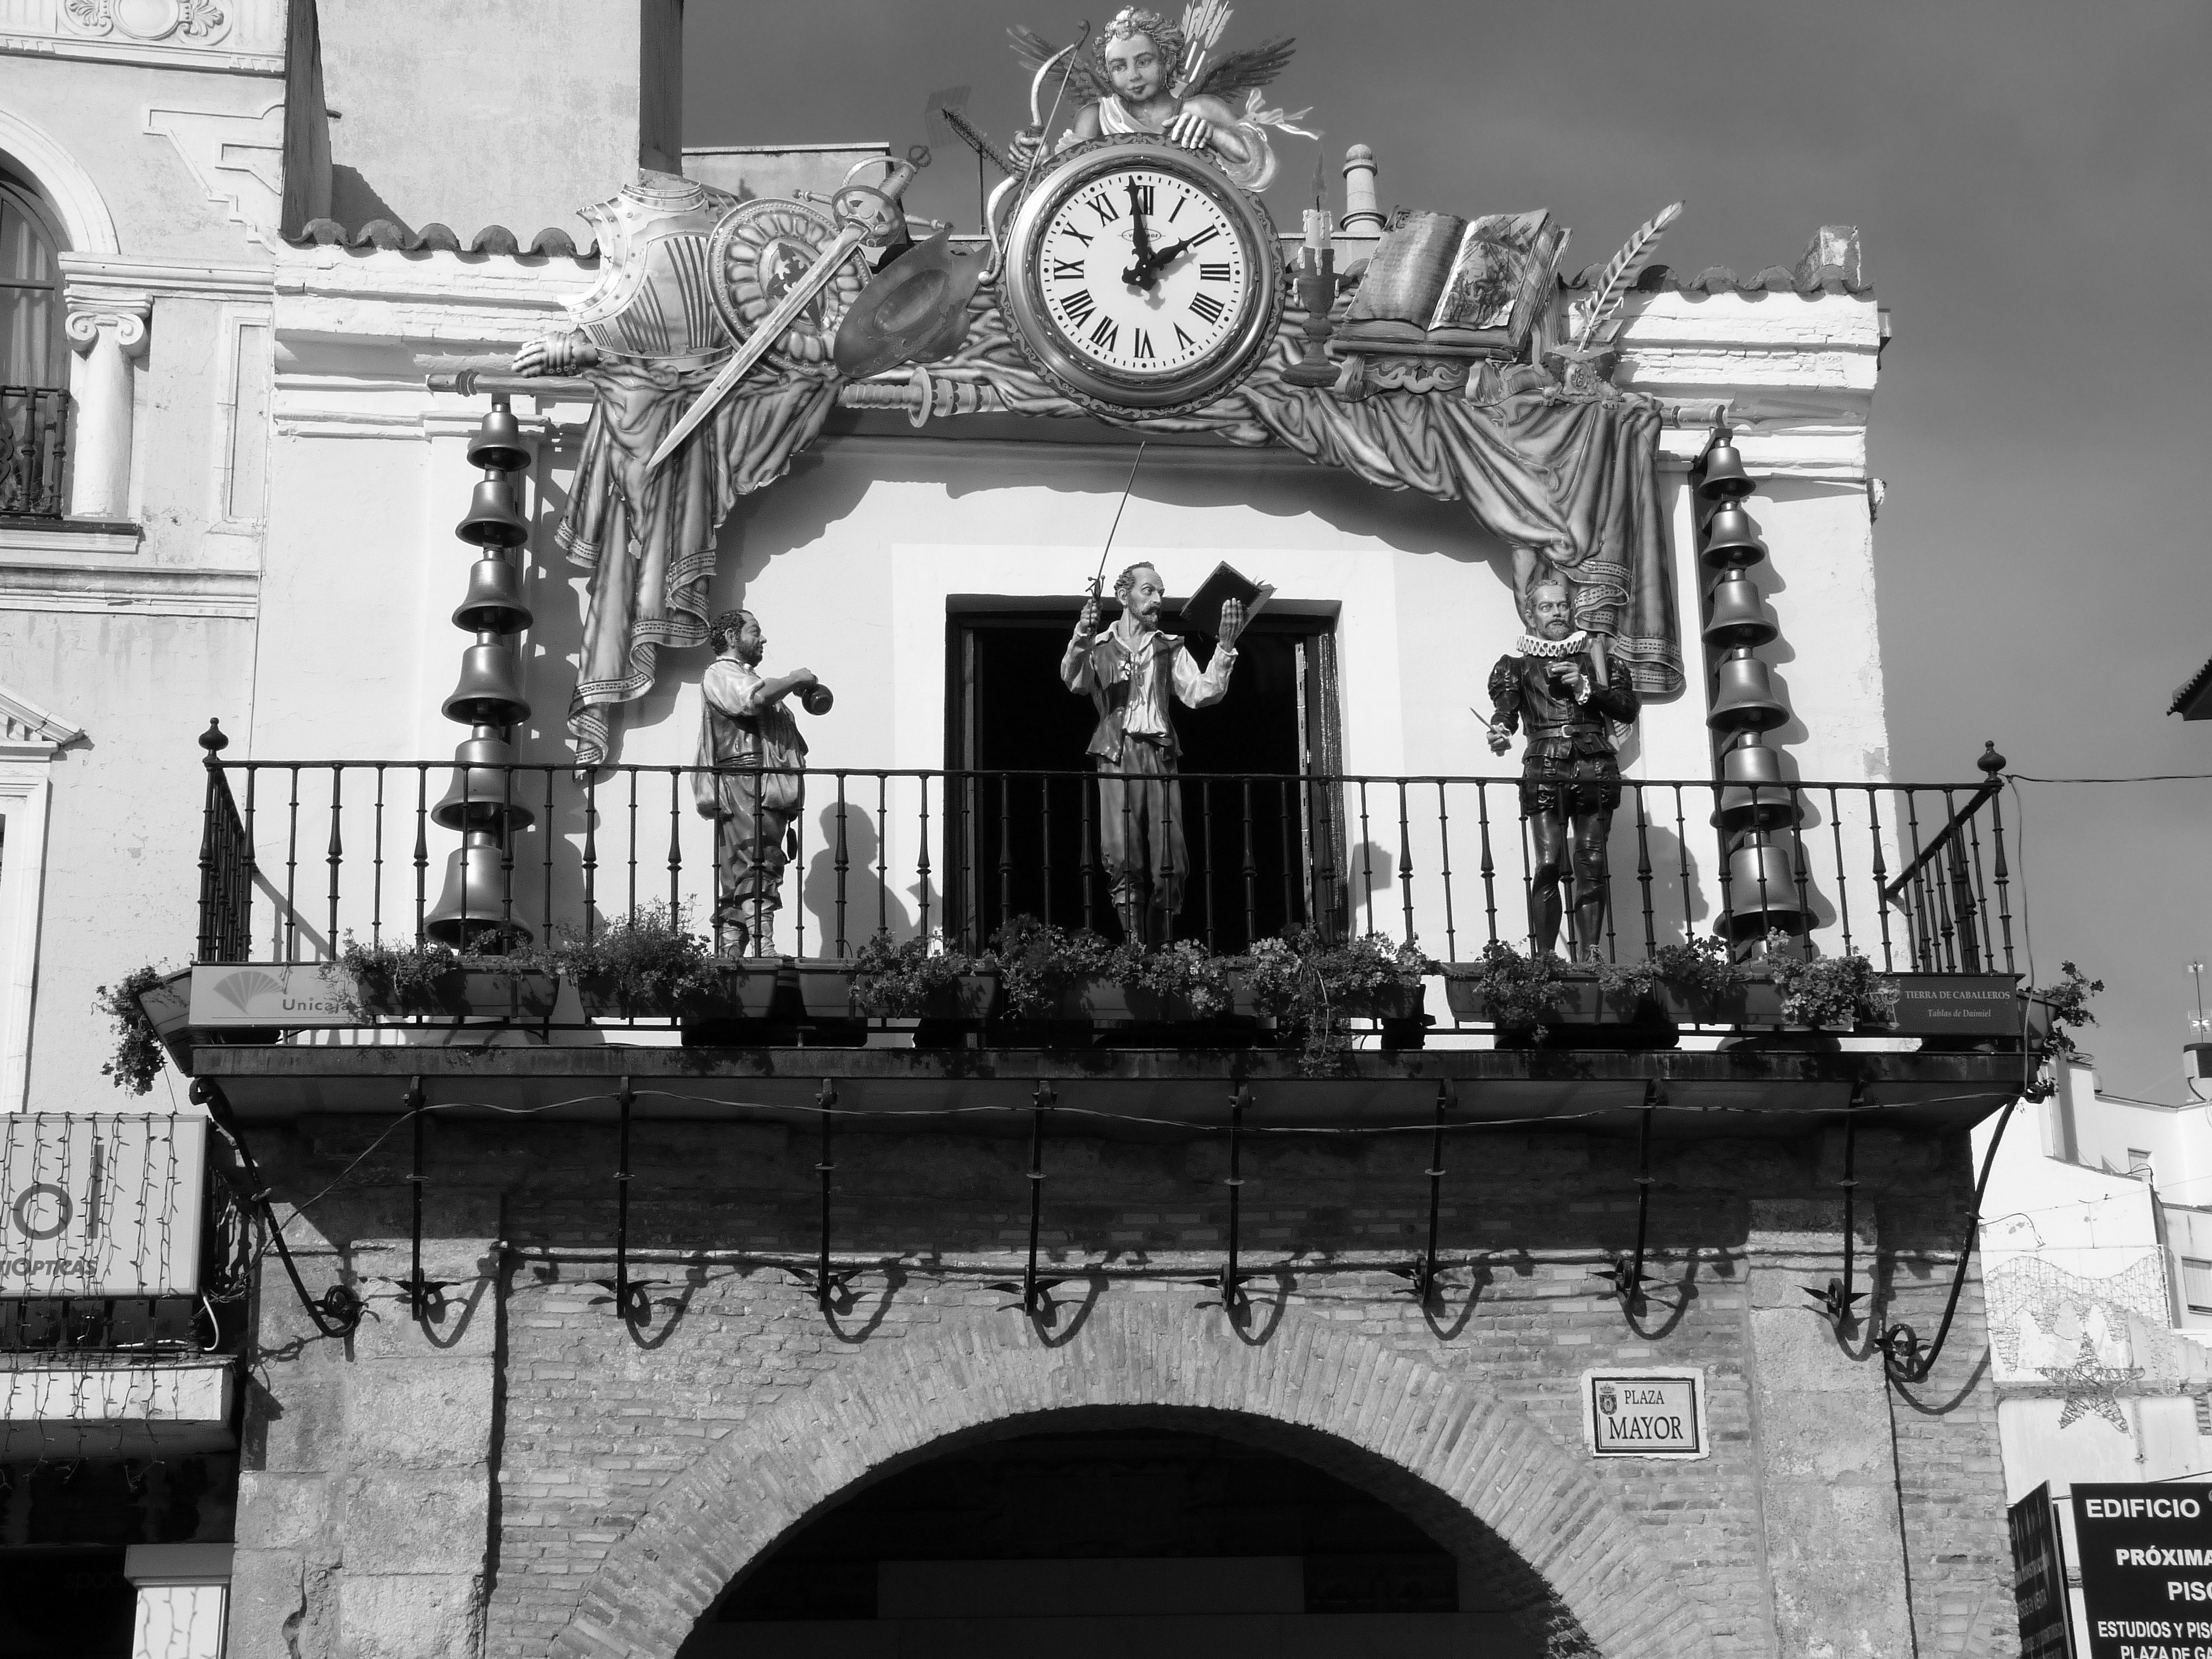
\includegraphics[width=5.5cm]{clockCRbw}
%		\label{fig:clockCRbw}
%	}
%	\caption[Comparación jpg color y niveles de gris]{El reloj de la Plaza Mayor (cortesía de J.~Salido)}
%	\label{fig:clock}
%\end{figure}


% Ejemplo:
% ============
%Aquí se muestra cómo se emplean subfiguras. Se pueden añadir cuantas subfiguras se desee, de modo que si no caben a la par LaTeX las ubicará en varias filas. Esta colocación en varias filas se puede provocar añadiendo \\ (saltos de línea). Las subfiguras también se pueden emplear en las refs. cruzadas. El título de la figura también admite un título corto para la lista de figuras.
\begin{figure}[hbt]
	\centering
	\begin{subfigure}[b]{0.4\linewidth}
		\centering
		\includegraphics[width=0.8\linewidth]{clockCR}
		\caption{Imagen jpg en color}\label{fig:clockCR}
	\end{subfigure}
	\begin{subfigure}[b]{0.4\linewidth}
		\centering
		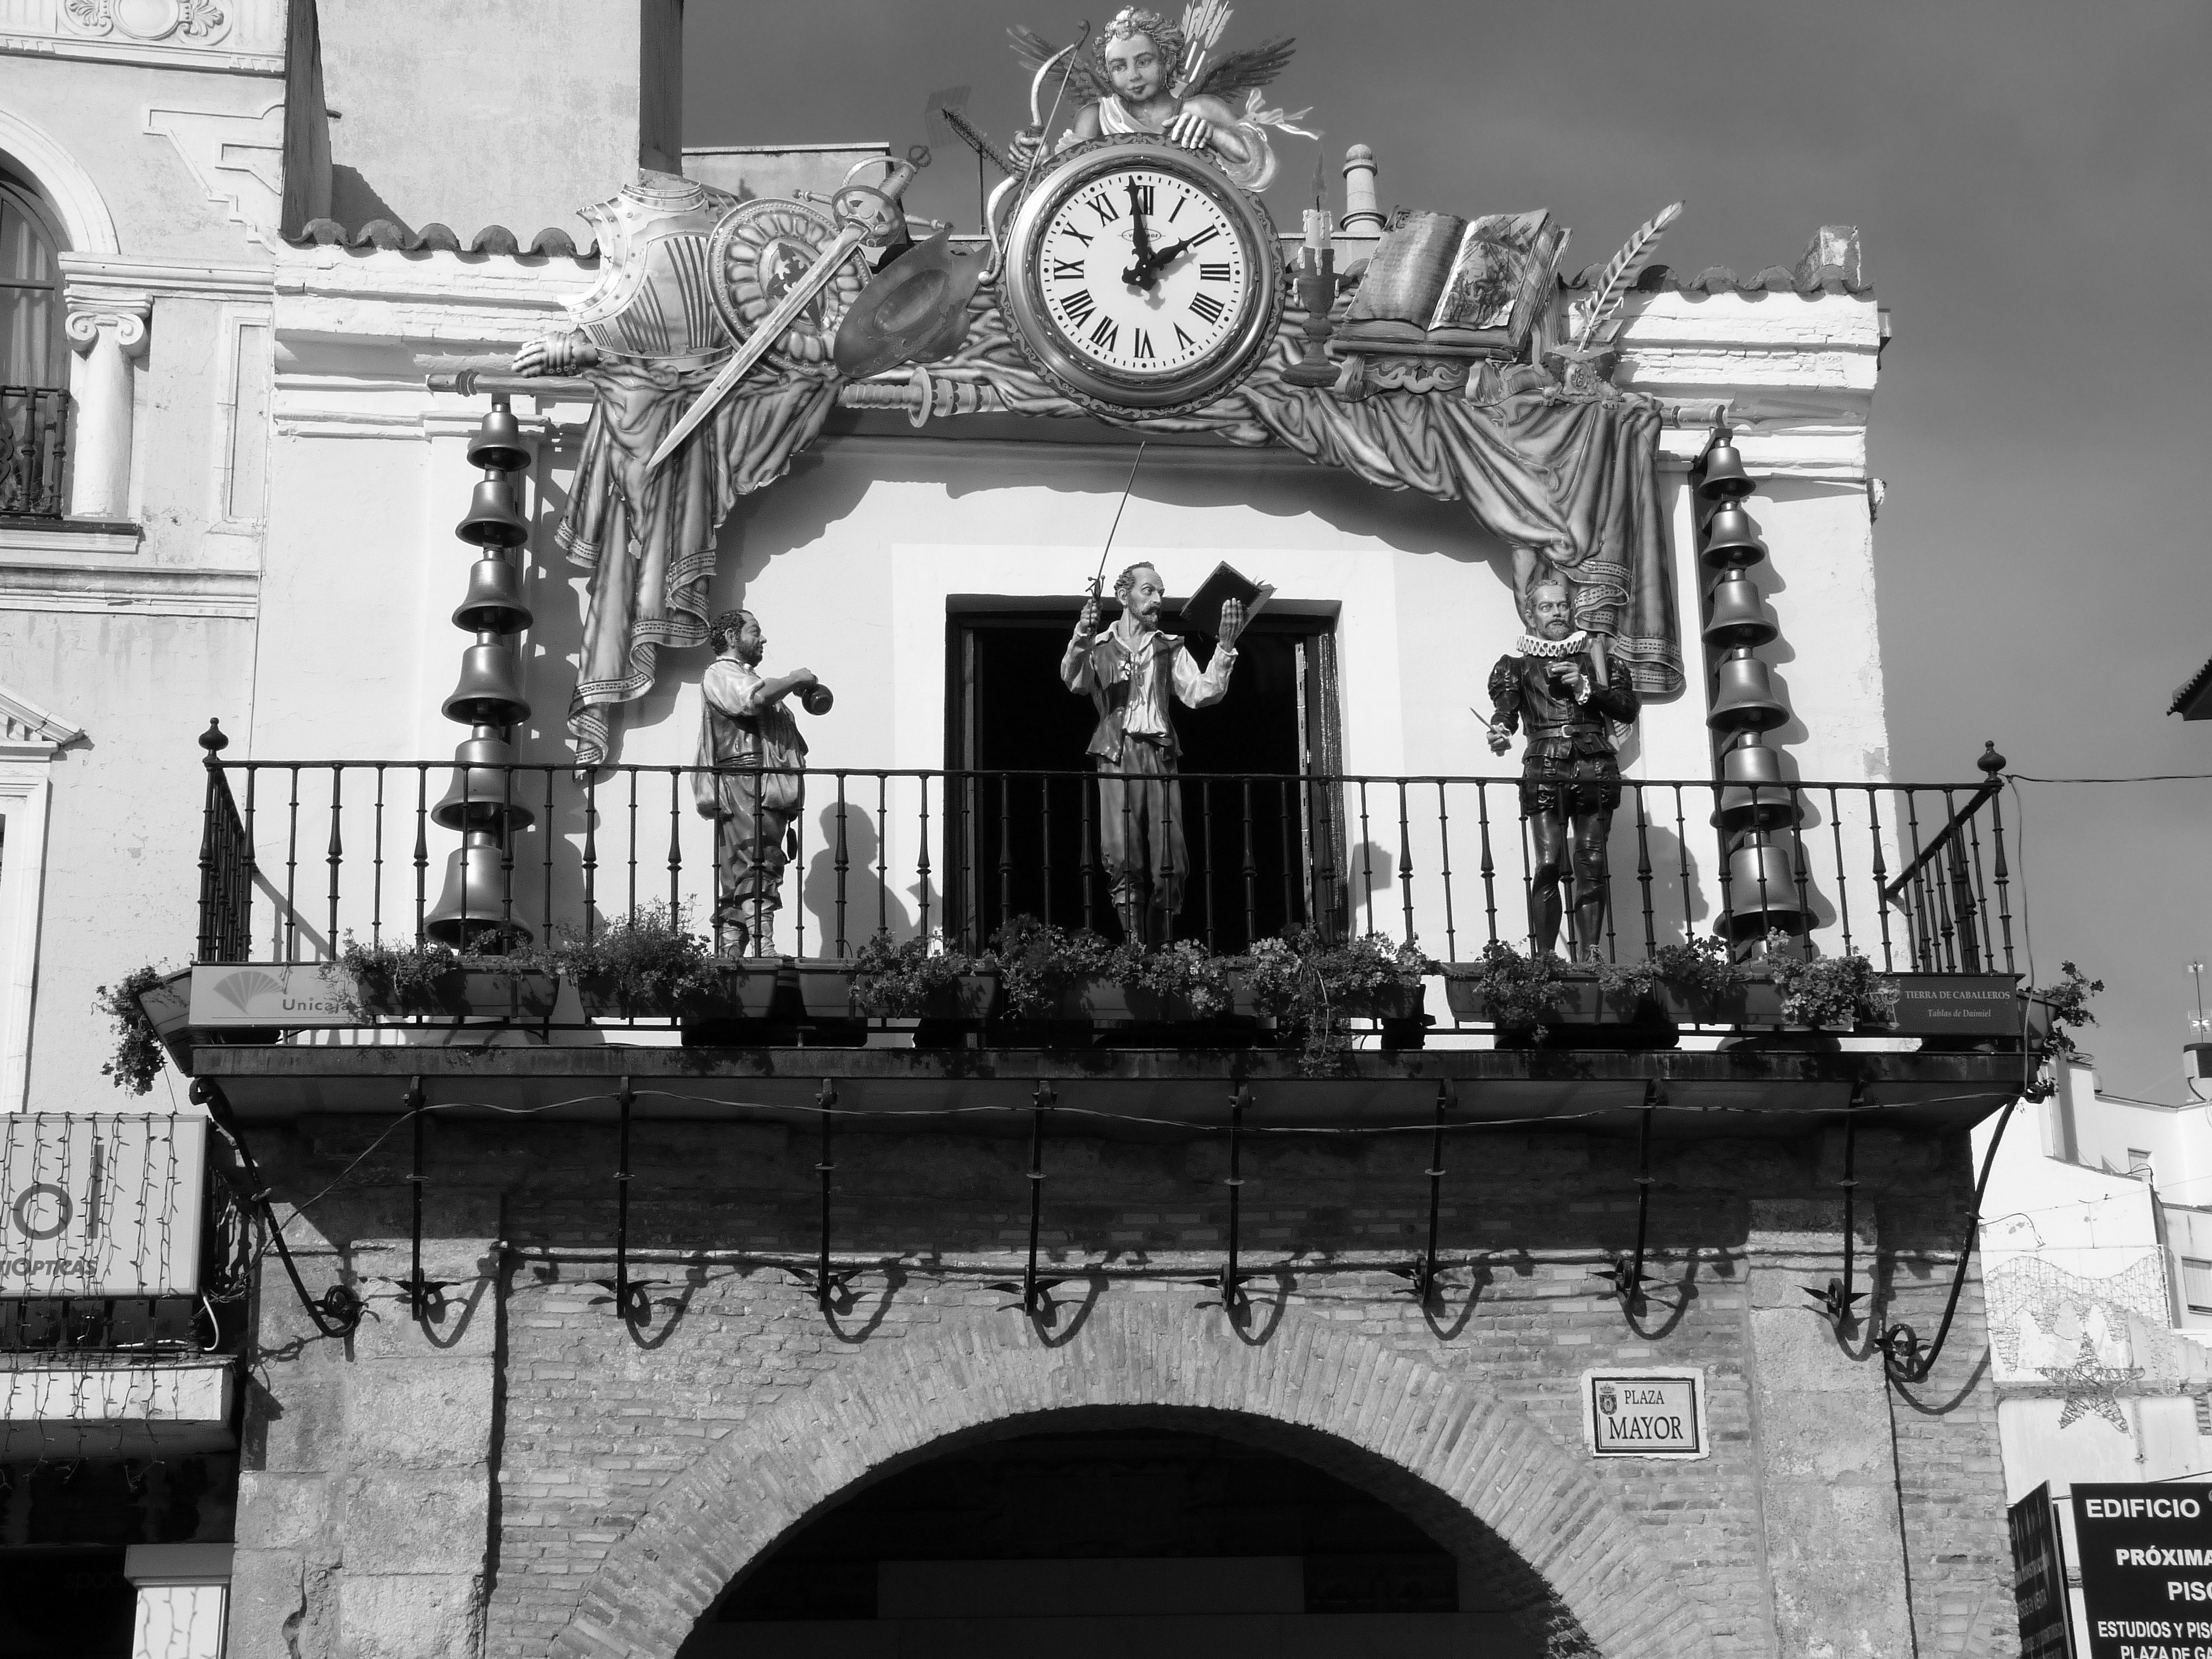
\includegraphics[width=0.8\linewidth]{clockCRbw}
		\caption{Imagen jpg en niveles de gris}\label{fig:clockCRbw}
	\end{subfigure}
	\caption[Comparación jpg color y niveles de gris]{Ej. de paquete \texttt{subcaption} mostrando el reloj de la Plaza Mayor (cortesía de J.~Salido)}
	\label{fig:clock}
\end{figure}



% Ejemplo:
% ============
%Aquí se muestra cómo incluir una figura compuesta por subfiguras. Para montarlas se emplearon los programas PhotoFiltre y Powerpoint. Primero se redujo el tamaño original de las imágenes para que ocupasen menos memoria y después se montaron con Powerpoint una junto a otra dejando un espacio en blanco entre ellas. Este montaje se exporto a Photofiltre para salvarlo en el formato final.
\begin{figure}[hbt]
	\centering
		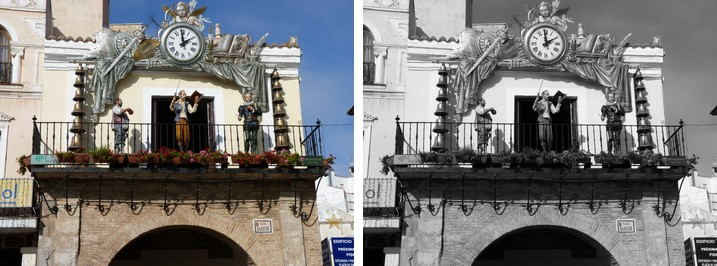
\includegraphics[width=0.6\linewidth]{2clockCR}
		\caption[Varias imágenes como una]{El reloj de la Plaza Mayor en color (izda.) y niveles de gris (dcha.)}
	\label{fig:2clock}
\end{figure}


Siempre que se tenga un fichero de imagen (mapa de bits) con un fondo blanco u otro color plano, debería intentarse transformar en una imagen con fondo transparente convirtiéndola al formato \texttt{.png} (véase ejemplo en la Fig.~\ref{fig:lion}).


% Ejemplo:
% ============
\begin{figure}[hbt]
	\centering
  	\begin{subfigure}[b]{0.4\linewidth}
  		\centering
		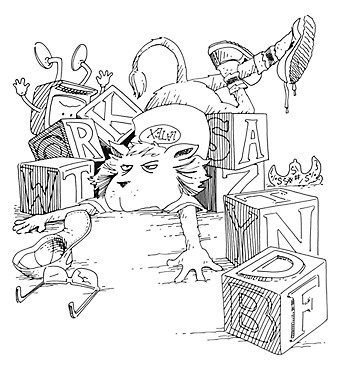
\includegraphics[width=6cm]{lionL.jpg}
		\caption{Imagen como jpg}\label{fig:lionLjpg}
  	\end{subfigure}
  	\begin{subfigure}[b]{0.4\linewidth}
  		\centering
		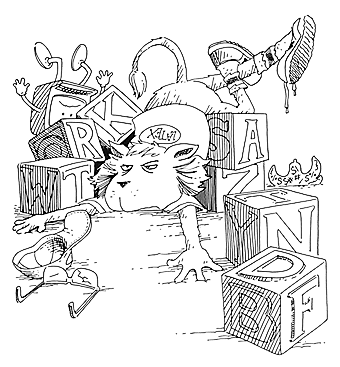
\includegraphics[width=6cm]{lionL.png}
		\caption{Imagen como png con fondo transparente}\label{fig:lionpng}
  	\end{subfigure}
  	\caption[Comparación jpg y png con transparencia]{Comparativa de formatos bitmap (cortesía de D.~Wright)}
	\label{fig:lion}
\end{figure}

Si se desea es posible usar imágenes en color. Esto es muy conveniente para documentos electrónicos que se van a visualizar en la pantalla de un computador. Sin embargo, para documentos que serán impresos hay que tener presente algunos aspectos del color. 

En la Fig.~\ref{fig:clock} se muestra un ejemplo de empleo de subfiguras. En dicho ejemplo se muestra dos versiones de la misma imagen, la subfigura~\ref{fig:clockCR} es una versión en color (tal cual se tomó la fotografía original) y la sufigura~\ref{fig:clockCRbw} muestra la misma imagen transformada en niveles de gris.

La Fig.~\ref{fig:lion} muestra un ejemplo de subfiguras mostrando la misma figura en formatos \texttt{.jpg} y \texttt{.png} en la que el fondo blanco se ha convertido en transparente. 

En la Fig.~\ref{fig:escudo} se pueden comparar los resultados obtenidos cuando la figura se inserta en formato vectorial (escalable) y cuando se hace como mapa de bits (no escalable). En este ejemplo se muestran dos versiones para el escudo de la Ingeniería Informática (cortesía de CRySoL).\footnote{El escudo basado en el núcleo de ferrita que acompaña la distribución de este documento ha sido realizado por Francisco Moya, David Villa e Ignacio Díez y su inclusión en el documento final debe respetar los derechos de la licencia CC BY-SA 3.0 con la que se distribuye.}


% Ejemplo:
% ============
\begin{figure}[hbt]
	\centering
	\begin{subfigure}[b]{0.4\linewidth}
		\centering
		
\includegraphics[width=3.5cm]{escudoInfBW.pdf}
		\caption{Gráfico vectorial PDF}\label{fig:escudoPDF}
	\end{subfigure}
	\begin{subfigure}[b]{0.4\linewidth}
		\centering
		
\includegraphics[width=3.8cm]{escudoInfBW.png}
		\caption{Gráfico png}\label{fig:escudoPNG}
	\end{subfigure}
	\caption[Comparación PDF y png]{Comparando distintos formatos para el escudo de Informática (cortesía de CRySoL)}
	\label{fig:escudo}
\end{figure}


Cuando se trabaja con figuras hay que tener mucho cuidado con emplear imágenes de Internet sin tener la seguridad de los términos de uso de las mismas (i.e.\ ). Con mucha frecuencia, de forma inadvertida, se violan los derechos de uso cometiendo, incluso, un delito. Por este motivo recomiendo recurrir a librerías de dominio público que permiten el uso de las imágenes y \emph{clip arts} sin restricciones, como por ejemplo Open ClipArt,\footnote{\url{http://openclipart.org/}} la página de galerías en el sitio de Inkscape\footnote{\url{http://wiki.inkscape.org/wiki/index.php/Galleries}} y Wikimedia Commons.\footnote{\url{http://commons.wikimedia.org/}} El derecho a cita permite la reproducción de figuras, sujetas a derechos restrictivos de distribución, en ámbitos académicos. Sin embargo, siempre debería incluirse en el pie de la figura la atribución de autoría y la licencia que se aplica a la distribución de la misma (no confundir con la licencia de nuestro documento). En cualquier caso debería investigarse la licencia de uso de la figura puesto que en algunos casos (p.ej.\ banco de imágenes de la \textsc{nasa}) el autor señala cómo debe realizarse la atribución de autoría. En ningún caso puede incluirse una figura ajena sin atribución, sin importar si es de dominio público o distribuida con una licencia permisiva. Se asume que toda figura que no se atribuye a su legítimo autor es de nuestra autoría.



\newpage
\subsection{Imágenes a las que se añaden gráficos}
En ocasiones es necesario recurrir a capturas de pantalla sobre las que es preciso realizar alguna anotación gráfica, por ejemplo añadiendo flechas y bloques de texto. Este es un caso que puede aparecer cuando se explica el funcionamiento de un programa informático (p.~ej.\ un manual). La captura siempre se debe realizar al mayor tamaño posible sobre la pantalla y se debe salvar en formato \texttt{.png}. Generalmente las herramientas de captura permiten la edición de la captura añadiéndole elementos gráficos e incluso texto. En este caso los elementos añadidos 
forman parte del fichero \texttt{.png} y por tanto son definidos como mapa de bits. Si se desea mantener las características escalables de los elementos gráficos, éstos deben ser añadidos mediante algún programa de edición vectorial (p.~ej.\ 
\textsf{Inkscape}, \textsf{Dia}, \textsf{Visio}, etc.) y salvar el fichero resultante en formato \texttt{.pdf}. Las figs.~\ref{fig:texmk02} y \ref{fig:texmk03} muestran las diferencias en los dos procesos mencionados.

% Ejemplo:
% ============
\begin{figure}[hbt]
	\centering
	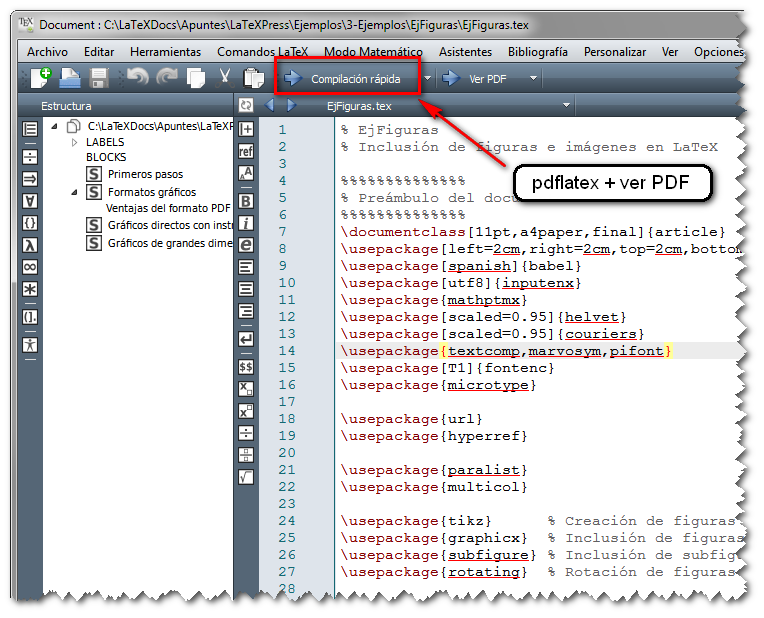
\includegraphics[width=0.5\linewidth]{texmk02} 
	\caption[Captura con gráfico en \texttt{png}]{Captura de pantalla con añadido gráfico en formato \texttt{png}}
	\label{fig:texmk02}
\end{figure}

% Ejemplo:
% ============
\begin{figure}[hbt]
	\centering
	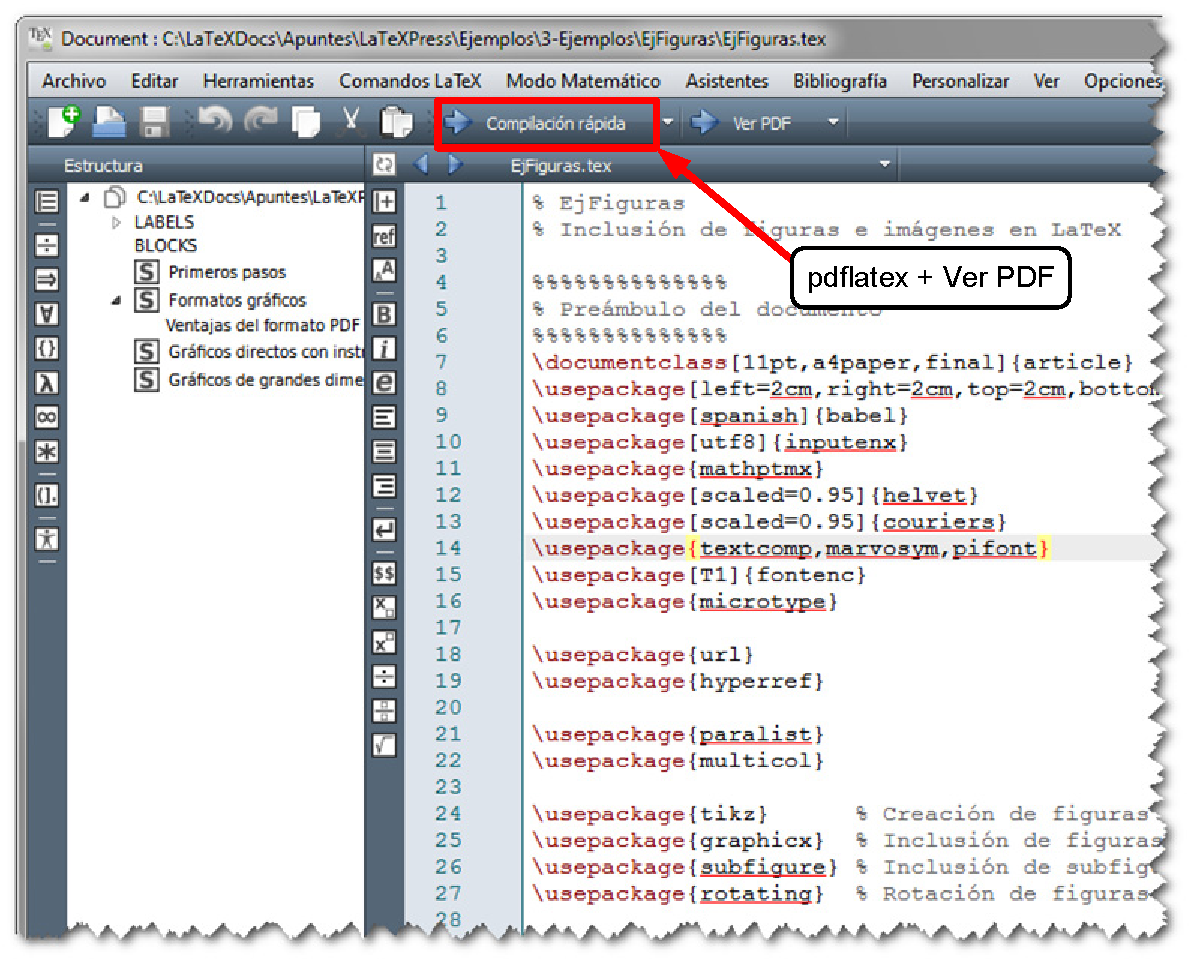
\includegraphics[width=0.5\linewidth]{texmk03} 
	\caption[Captura con gráfico en \texttt{pdf}]{Captura de pantalla con añadido gráfico en formato \texttt{pdf}}
	\label{fig:texmk03}
\end{figure}




\newpage
\subsection{Inclusión de páginas individuales de un PDF multipágina}

La Fig.~\ref{fig:visio_mp} nos muestra el procedimiento para usar los ficheros PDF multipágina para incluir el gráfico de una página concreta.

% Ejemplo:
% ============
\begin{figure}[hbt]
	\centering
	\includegraphics[page=2,width=0.5\linewidth]{visio_mp} 
	\caption[Gráfico de Visio multipágina]{Figura vectorial generada con Microsoft Visio en un fichero multipágina}
	\label{fig:visio_mp}
\end{figure}




\section{Gráficos de grandes dimensiones}
Cuando se presenta la necesidad de incluir un gráfico demasiado grande para el tamaño de la página una opción muy apropiada es la impresión del gráfico en modo apaisado en una página aparte. Este efecto se consigue con el entorno \texttt{sidewaysfigure} proporcionado por el paquete \texttt{rotating}. La Fig.~\ref{fig:sideways} muestra un ejemplo del entorno citado con un gráfico PDF.

% Ejemplo:
% ============
\begin{sidewaysfigure}
	\centering
	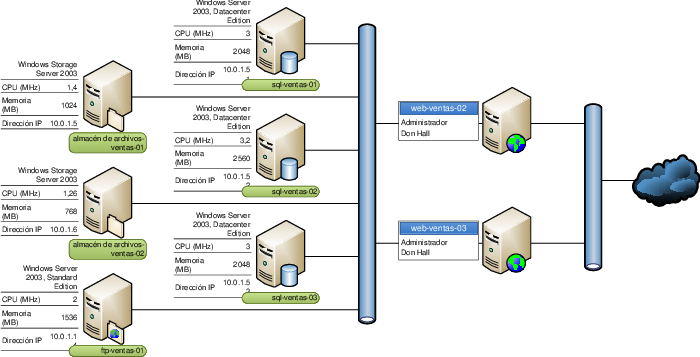
\includegraphics[width=19cm]{network} 
	\caption[Gráfico de apaisado Visio]{Figura vectorial con impresión apaisada}
	\label{fig:sideways}
\end{sidewaysfigure}
%	TO DO: Incluir comentarios sobre la orientación en modo apaisado. 
%	Consultar el contenido de la dirección: 
%	http://texblog.wordpress.com/2007/11/10/landscape-in-latex/
%	http://texblog.wordpress.com/tag/landscape/



\newpage
\section{Gráficos directos con instrucciones \TeX}
Además de los aspectos comentados aquí sobre la inclusión de imágenes y gráficos, \LaTeX{} dispone de una infinidad de recursos que pueden por sí mismo ser objeto de un curso. La figura~\ref{fig:carrito} se muestra la capacidad de realización de gráficos mediante instrucciones directas de \TeX{}. Un paquete muy poderoso en la generación de gráficos dentro de entornos \LaTeX{} es \texttt{tikz} (ver Fig.~\ref{fig:tikz}). La cantidad y variedad de gráficos que puede realizar es muy numerosa\footnote{Muchos ejemplos de uso en \url{http://www.texample.net/tikz/examples/}, y en especial los apartados dedicados a \href{http://www.texample.net/tikz/examples/area/electrical-engineering/}{ingeniería eléctrica} e \href{http://www.texample.net/tikz/examples/area/computer-science/}{informática}, junto con la página de web \href{https://www.kleemans.ch/diagrams-for-logic-in-latex}{<<Diagrams for Logic in \LaTeX>>}} aunque su uso requiere un conocimiento muy profundo y no es recomendable para principiantes.


% Ejemplo:
% ============
% Gráfico realizado con instrucciones directas de TeX, en este caso además el gráfico se ha incluido en un entorno figure para que sea tratado como un objeto flotante.
\begin{figure}[hbt]
	\centering
	\newcounter{cms}
	\setlength{\unitlength}{1mm}
	\begin{picture}(50,39)
	\put(15,20){\circle{6}} \put(30,20){\circle{6}}
	\put(15,20){\circle*{2}}\put(30,20){\circle*{2}}
	\put(10,24){\framebox(25,8){
			$I = \! \int_{-\infty}^\infty f(x)\,dx$
	}}
	\put(10,32){\vector(-2,1){10}}
	\put(0,7){\makebox(0,0)[bl]{cm}}
	\multiput(10,7)(10,0){5}{%
		\addtocounter{cms}{1}%
		\makebox(0,0)[b]{\thecms}}
	\multiput(1,0)(1,0){49}{\line(0,1){2.5}}
	\multiput(5,0)(10,0){5}{\line(0,1){3.5}}
	\thicklines
	\multiput(0,0)(10,0){6}{\line(0,1){5}}
	\put(0,0){\line(1,0){50}}
	\end{picture}
	\caption[Ejemplo de gráfico \LaTeX{}]{Figura realizada directamente con instrucciones \TeX{}}\label{fig:carrito}
\end{figure}


% Ejemplo:
% ============
% Gráfico realizado con paquete tikZ, en este caso además el gráfico se ha incluido en un entorno figure para que sea tratado como un objeto flotante.
\begin{figure}[hbt]
	\centering
	{\shorthandoff{>}
		\begin{tikzpicture}[>=stealth]
		\draw [->] (-1.5,0) -- (1.5,0);
		\draw [->] (0,-1.5) -- (0,1.5);
		\shadedraw (0.5,0.5) circle (0.5cm);
		%Relleno
		\filldraw[fill=red,even odd rule]
		(-1,-1) rectangle (0,0)
		(-0.5,-0.5) circle (0.4cm);
		\draw[->] (-0.9,-0.2) -- +(0,1)
		[above] node{Relleno};
		\end{tikzpicture}
	}
	\caption[Ejemplo de gráfico con Ti\textit{K}Z]{Figura realizada con paquete \texttt{tikz}}\label{fig:tikz}
\end{figure}






\end{document}